% TikZ Diagram: Metric Tensor Components Visualization
% 4×4 matrix with physical interpretation of each element
% Pedagogical breakdown inspired by Lions Commentary annotation style

\begin{figure}[htbp]
\centering
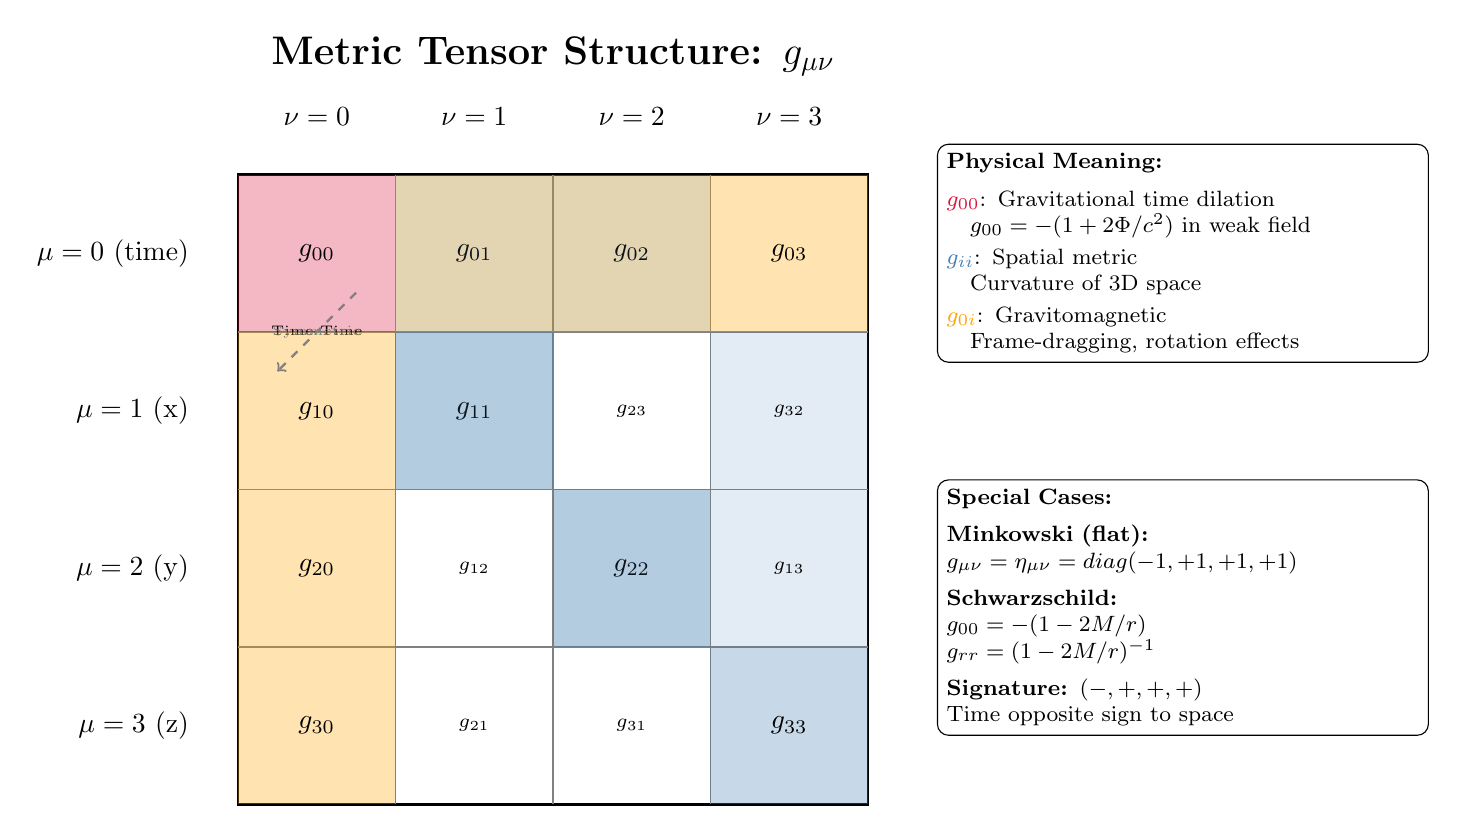
\begin{tikzpicture}[scale=1.0]
  
  % Define colors for different component types
  \definecolor{timecolor}{RGB}{220,20,60}      % Red for time-time
  \definecolor{spacecolor}{RGB}{70,130,180}    % Blue for space-space
  \definecolor{mixedcolor}{RGB}{255,165,0}     % Orange for time-space
  \definecolor{labelcolor}{RGB}{50,50,50}      % Dark gray for labels
  
  % Matrix outline
  \draw[thick] (0,0) rectangle (8,8);
  
  % Grid lines
  \foreach \i in {2,4,6} {
    \draw[gray] (0,\i) -- (8,\i);
    \draw[gray] (\i,0) -- (\i,8);
  }
  
  % g_00 component (time-time)
  \fill[timecolor, opacity=0.3] (0,6) rectangle (2,8);
  \node at (1,7) {$g_{00}$};
  \node[below, font=\tiny] at (1,6.2) {Time-Time};
  
  % g_0i components (time-space, off-diagonal)
  \fill[mixedcolor, opacity=0.3] (2,6) rectangle (4,8);
  \node at (3,7) {$g_{01}$};
  \fill[mixedcolor, opacity=0.3] (4,6) rectangle (6,8);
  \node at (5,7) {$g_{02}$};
  \fill[mixedcolor, opacity=0.3] (6,6) rectangle (8,8);
  \node at (7,7) {$g_{03}$};
  
  % g_i0 components (space-time, symmetric)
  \fill[mixedcolor, opacity=0.3] (0,4) rectangle (2,6);
  \node at (1,5) {$g_{10}$};
  \fill[mixedcolor, opacity=0.3] (0,2) rectangle (2,4);
  \node at (1,3) {$g_{20}$};
  \fill[mixedcolor, opacity=0.3] (0,0) rectangle (2,2);
  \node at (1,1) {$g_{30}$};
  
  % g_ij components (space-space, diagonal)
  \fill[spacecolor, opacity=0.3] (2,4) rectangle (4,6);
  \node at (3,5) {$g_{11}$};
  \fill[spacecolor, opacity=0.3] (4,2) rectangle (6,4);
  \node at (5,3) {$g_{22}$};
  \fill[spacecolor, opacity=0.3] (6,0) rectangle (8,2);
  \node at (7,1) {$g_{33}$};
  
  % Off-diagonal space-space components
  \foreach \i/\j in {2/4, 2/6, 4/6, 4/2, 6/2, 6/4} {
    \fill[spacecolor, opacity=0.15] (\i,\j) rectangle (\i+2,\j+2);
  }
  \node[font=\scriptsize] at (3,3) {$g_{12}$};
  \node[font=\scriptsize] at (5,5) {$g_{23}$};
  \node[font=\scriptsize] at (7,3) {$g_{13}$};
  \node[font=\scriptsize] at (3,1) {$g_{21}$};
  \node[font=\scriptsize] at (5,1) {$g_{31}$};
  \node[font=\scriptsize] at (7,5) {$g_{32}$};
  
  % Axis labels
  \node[left] at (-0.5,7) {$\mu=0$ (time)};
  \node[left] at (-0.5,5) {$\mu=1$ (x)};
  \node[left] at (-0.5,3) {$\mu=2$ (y)};
  \node[left] at (-0.5,1) {$\mu=3$ (z)};
  
  \node[above] at (1,8.5) {$\nu=0$};
  \node[above] at (3,8.5) {$\nu=1$};
  \node[above] at (5,8.5) {$\nu=2$};
  \node[above] at (7,8.5) {$\nu=3$};
  
  % Symmetry indicator
  \draw[->, thick, dashed, gray] (1.5,6.5) -- (0.5,5.5);
  \node[gray, font=\tiny] at (1,6) {Symmetric};
  
  % Physical interpretation annotations (right side)
  \node[draw, rounded corners, fill=white, align=left, font=\footnotesize, text width=6cm] at (12,7) {
    \textbf{Physical Meaning:}\\[4pt]
    \textcolor{timecolor}{\textbf{$g_{00}$}}: Gravitational time dilation\\
    \quad $g_{00} = -(1 + 2\Phi/c^2)$ in weak field\\[2pt]
    \textcolor{spacecolor}{\textbf{$g_{ii}$}}: Spatial metric\\
    \quad Curvature of 3D space\\[2pt]
    \textcolor{mixedcolor}{\textbf{$g_{0i}$}}: Gravitomagnetic\\
    \quad Frame-dragging, rotation effects
  };
  
  % Minkowski limit annotation (bottom right)
  \node[draw, rounded corners, fill=white, align=left, font=\footnotesize, text width=6cm] at (12,2.5) {
    \textbf{Special Cases:}\\[4pt]
    \textbf{Minkowski (flat):}\\
    $g_{\mu\nu} = \eta_{\mu\nu} = \text{diag}(-1,+1,+1,+1)$\\[4pt]
    \textbf{Schwarzschild:}\\
    $g_{00} = -(1-2M/r)$\\
    $g_{rr} = (1-2M/r)^{-1}$\\[4pt]
    \textbf{Signature:} $(-,+,+,+)$\\
    Time opposite sign to space
  };
  
  % Title
  \node[font=\Large\bfseries] at (4,9.5) {Metric Tensor Structure: $g_{\mu\nu}$};
  
\end{tikzpicture}
\caption{Structure of the metric tensor $g_{\mu\nu}$ showing the physical interpretation of each component. The \textcolor{timecolor}{red} element $g_{00}$ encodes gravitational time dilation, \textcolor{spacecolor}{blue} diagonal spatial elements $g_{ii}$ represent spatial curvature, and \textcolor{mixedcolor}{orange} off-diagonal $g_{0i}$ terms describe frame-dragging and rotation. The tensor is symmetric ($g_{\mu\nu} = g_{\nu\mu}$), reducing 16 components to 10 independent degrees of freedom. In flat Minkowski spacetime, all off-diagonal terms vanish and diagonal elements are $\pm 1$.}
\label{fig:prelim:metric-structure}
\end{figure}
